\documentclass[10pt]{article}
\usepackage {fullpage}
\usepackage{graphicx}
\setlength{\parskip}{1em}
\usepackage{amsmath}
\usepackage{amsfonts}
\usepackage{amssymb}
\usepackage{listings}
\lstset{language=Matlab}
\lstset{tabsize=2}

\begin{document}
		\title{Report}
		\author{Hoang Duc Viet}
		\date{\today}
		\maketitle

\newpage
%\tableofcontents
\newpage
\section{Noise}
Noises always appear around our lives everywhere. For example, noise from vehicles, factories or construction sites... Moreover noise also appears in the images. First, we are going to research about images noise.

Image noise can be appear by the sensor and circuitry from scanner or digital camera. Moreover, film grain and noise of an ideal photon detector are also cause. From above causes , brightness or color information in images will be change. Image noise is unlike by product of image capture that have many different information.

Next, it is quality of camera. Although camera technology is very improve over the past decade, it still has not totally remove noise for images. So now, researchers still find to way which improve about camera to help us have image is better.   


Noise can appear in our photo for different reasons. Noise signal increases with the light signal when high ISO is used, therefore our camera will capture more light to illuminate the scene, but graininess will be more apparent. When an image sensor became heats up, photons separate from the iamges and destroy other images. Long exposures also give our image greater risk of showing image noise, since the sensor is left open to gather more image data and this includes electrical noise.

Noise is the cause of errors from image when in pixel values that do not reflect the true intensities of the real scene. There are 3 types of image noise as below :

\subsection{Fixed Pattern}
Fixed pattern noise appear during extremely long exposures. So when the camera is working for long periods of time and it heats up, the sensor starts to produce these strange dots of color in our image. And our camera is hotter, more fixed pattern noise will appear.
\begin{center}
	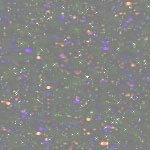
\includegraphics{fix.png}
\end{center}


\subsection{Random Noise}
Random noise maybe the most common image noise. Random noise appear whenever we’re using high ISO values.

Cameras has good at reducing the amount of random noise that is seen in photographs through technology. The noise reduction feature on some cameras which remove random noise. So when technology continues to improve, we can shoot in low light situation. 

\begin{center}
	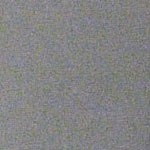
\includegraphics{random.png}
\end{center}

\subsection{Banding Noise}
Banding noise is dependent on what type of camera we are using. With high end camera, we have never seen banding noise. Some banding noise will appear when lower quality photograph are shot with higher ISO value.

There are causes help banding noise appear: in the dark of photos or increase exposure too much and digitally make a photograph too bright . We may also see more banding noise in certain white balances.


\begin{center}
	
\includegraphics{banding.png}
\end{center}


\section{Noise Removal}

Noise removal is very important task in image processing. It will help image restoration is to remove the noise from the image in such a way that the original image is the best quality. In modern digital image processing, data denoising is a hard problem and it used to application areas. Noise removal is popular solution for photography or improve the  image was degraded.


\subsection{Spatial Filtering}
Spatial filtering is a form of finite impulse response (FIR) filtering. The filter is a mask of weights arranged in a rectangular pattern. It mean that sliding the mask along the image and performing a multiply and accumulate operation on the pixels covered by the mask.


Filtering is technique which can be decreasing or increasing an image. It's the processed value for the current pixel which depends on both itself and surrounding pixels.
So filtering is a neighborhood operation, it mean that the value of any given pixel in the output image is determined by applying some algorithm to the values of the pixels in the neighborhood of the corresponding input pixel. A pixel's neighborhood is some set of pixels, defined by their locations relative to that pixel. 

Follow Image Processing,  there are 4 type of filtering :

\begin{itemize}
	\item  Median Filter.

The median filter is a nonlinear digital filtering technique. So median filtering is very widely used in image processing and it preserves edges while removing noise under certain conditions.

	\item  Average Filter.
	
	The type of mean filtering is simply to replace each pixel value in an image with the mean('average') value of its neighbors, including itself. This has the effect of eliminating pixel values which are
	unrepresentative of their environment. Mean filtering as a convolution filter.
	
	\item  Gaussian Filter.
	
	In electronics and signal processing, filter whose impulse response is a Gaussian function (or an approximation to it). Gaussian filters have feature of having no overshoot to a step function input while minimizing the rise and fall time.

	\item Wiener Filter
	
	The main aim of this technique is to filter out noise that has corrupted the signal. It is kind of statistical approach. For the designing of this filter one should know the spectral properties of the original signal ,the noise and linear time-variant filter whose output should be as close as to the original as possible. The Wiener filter minimizes the mean square error between the estimated random process and the desired process.
	



\end{itemize}

 \subsection{Original Image }
First, we are going to read and show original image as below :
\begin{lstlisting}
I = imread('lena.tif');
F = imshow(I);
\end{lstlisting}

\textbf{Result:}
\begin{center}
	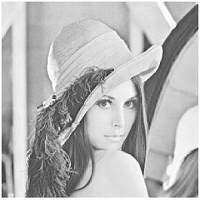
\includegraphics{lena1.png}

 Original Image
\end{center}

\subsection{Median Filter}
Median Filter is family of order filters. It has process : Replace the value of a pixel with the median value of the neighborhood.

$I_{median} = median(I[i,j])$  with $(i,j)\in neighborhood$

From theory above, we are going to build function for median filter :

\begin{lstlisting}
function F = median(I,w)
s=size(I);
for i=floor(w/2)+1:s(1)-floor(w/2)
	for j=floor(w/2)+1:s(2)-floor(w/2)
		for k=1:w
			for l=1:w
				vect(w*(k-1)+l)=I(i-floor(k/2)+2,j-floor(l/2)+2);
			end
		end
		B=sort(vect);
		I(i,j)=B(floor(size(B,2)/2)+1);
	end
end
figure;

imshow(I);

\end{lstlisting}


\textbf{Result:}

\begin{center}
	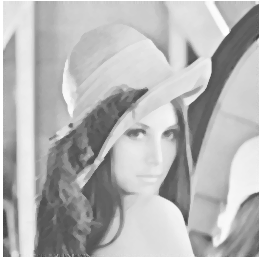
\includegraphics{median1.png}
	
	median x 7
\end{center}

\subsection{Average Filter}
\textbf{Feature: }
\begin{itemize}
	\item A spatial filter that applies to a neighborhood (local method).
	\item A linear filter, speaking as a convolution.
	\item A pixel is replaced by the average of itself and its neighbours.
	\item The neighborhood size determines the amount of smoothing.
    \item Equivalent to a filtering operation lowpass.
\end{itemize}

Average Filter have: 
\begin{center}
	Filter 3$\times$3

$\dfrac{1}{9}\begin{tabular}{|c|c|c|}
\hline 
1 & 1 & 1 \\ 
\hline 
1 & 1 & 1 \\ 
\hline 
1 & 1 & 1 \\ 
\hline 
\end{tabular}$ 	
\end{center}

\

\begin{center}
		Filter 5$\times$5
	
	$\dfrac{1}{25}\begin{tabular}{|c|c|c|c|c|}
		\hline 
		1 & 1 & 1 & 1 & 1 \\ 
		\hline 
		1 & 1 & 1 & 1 & 1 \\ 
		\hline 
		1 & 1 & 1 & 1 & 1 \\ 
		\hline 
		1 & 1 & 1 & 1 & 1 \\ 
		\hline 
		1 & 1 & 1 & 1 & 1 \\ 
		\hline 
	\end{tabular} $
\end{center}

\

\begin{center}
	Filter 7$\times$7

$\dfrac{1}{49}\begin{tabular}{|c|c|c|c|c|c|c|}
	\hline 
	1 & 1 & 1 & 1 & 1 & 1 & 1 \\ 
	\hline 
	1 & 1 & 1 & 1 & 1 & 1 & 1 \\ 
	\hline 
	1 & 1 & 1 & 1 & 1 & 1 & 1 \\ 
	\hline 
	1 & 1 & 1 & 1 & 1 & 1 & 1 \\ 
	\hline 
	1 & 1 & 1 & 1 & 1 & 1 & 1 \\ 
	\hline 
	1 & 1 & 1 & 1 & 1 & 1 & 1 \\ 
	\hline 
	1 & 1 & 1 & 1 & 1 & 1 & 1 \\ 
	\hline 
\end{tabular} $
\end{center}





\textbf{Function of Averaging filter:}
\begin{lstlisting}
function F=average(I)
s=size(I);
F_size=7;
F=double(zeros(s(1),s(2)));
	for i=floor(F_size/2)+1:s(1)- floor(F_size/2)
		for j=floor(F_size/2)+1:s(2)- floor(F_size/2)
			for k=1:F_size
				for l=1:F_size
					F(i,j)=F(i,j)+double(I(i+k-(floor(F_size/2)+1),j+l-(floor(F_size/2)+1)));
				end;
			end;
			F(i,j)=round(F(i,j)/(F_size*F_size));
			end;
		end;
F=uint8(F);
figure;
imshow(F);
\end{lstlisting}



\textbf{Result:}

\begin{center}
	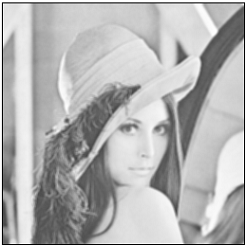
\includegraphics{a3x3.png}
	
	Filter $3\times3$
	
	 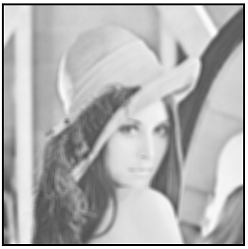
\includegraphics{a5x5.png}
	
	Filter $5\times5$
	
		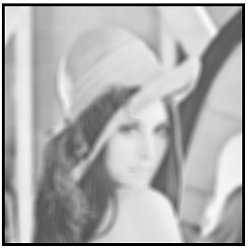
\includegraphics{a7x7.png}
	
Filter $7\times7$
\end{center}

\subsection{Gaussian Filter}

The Gaussian kernel in dimension 2:


$G(x,y) = \dfrac{1}{2\pi\sigma^2}\exp\left[-\dfrac{(x-\mu_x)^2+(y-\mu_y)^2}{2\sigma^2}\right ]$

\

Define the Gaussian mask:
%$$\mu = 0$$
%$$\sigma = 0.8$$
\begin{center}
	Filter 3$\times$3

$\dfrac{1}{16}\begin{tabular}{|c|c|c|}
	\hline 
	1 & 2 & 1 \\ 
	\hline 
	2 & 4 & 2 \\ 
	\hline 
	1 & 2 & 1 \\ 
	\hline 
\end{tabular} $
\end{center}

\begin{center}
	Filter 5$\times$5

$\dfrac{1}{273}\begin{tabular}{|c|c|c|c|c|}
	\hline 
	1 & 4 & 7 & 4 & 1 \\ 
	\hline 
	4 & 16 & 26 & 16 & 4 \\ 
	\hline 
	7 & 26 & 41 & 26 & 7 \\ 
	\hline 
	4 & 16 & 26 & 16 & 4 \\ 
	\hline 
	1 & 4 & 7 & 4 & 1 \\ 
	\hline 
\end{tabular}$ 
\end{center}

\begin{center}
	Filter 7$\times$7

$\dfrac{1}{1003}$\begin{tabular}{|c|c|c|c|c|c|c|}
	\hline 
	0 & 0 & 1 & 2 & 1 & 0 & 0 \\ 
	\hline 
	0 & 3 & 13 & 22 & 13 & 3 & 0 \\ 
	\hline 
	1 & 13 & 59 & 97 & 59 & 13 & 1 \\ 
	\hline 
	2 & 22 & 97 & 159 & 97 & 22 & 2 \\ 
	\hline 
	1 & 13 & 59 & 97 & 59 & 13 & 1 \\ 
	\hline 
	0 & 3 & 13 & 22 & 13 & 3 & 0 \\ 
	\hline 
	0 & 0 & 1 & 2 & 1 & 0 & 0 \\ 
	\hline 
\end{tabular} 
\end{center}



From theory above, we are going to build function for gaussian filter :
%\begin{lstlisting}
%function F = gaussian(I) 
%s=size(I);
%F_G=[1,2,1;2,4,2;1,2,1];
%F_size=3;
%F=double(zeros(s(1),s(2)));
	%for i=2:s(1)-1
		%for j=2:s(2)-1
			%for k=1:3
				%for l=1:3
					%F(i,j)=F(i,j)+double(I(i+k-2,j+l-2)*F_G(k,l));
					%end;
				%end;
					%F(i,j)=round(F(i,j)/(16));
				%end;
			%end;
%F=uint8(F);
%figure;
%imshow(F)
%\end{lstlisting}
\begin{lstlisting}
% Read an image
I = imread('lena.tif');
% Create the gaussian filter with hsize = [x y] and sigma = 2
G = fspecial('gaussian',[x y],2);
% Filter it
F = imfilter(I,G,'same');
% Display
imshow(F)	
\end{lstlisting}
\textbf{Result:}
\begin{center}
	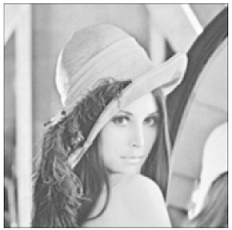
\includegraphics{b3x3.png}
	
	Filter $3\times3$
	
	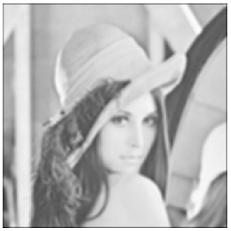
\includegraphics{b5x5.png}
	
	Filter $5\times5$
	
	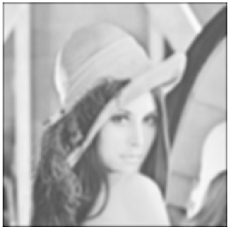
\includegraphics{b7x7.png}
	
	Filter $7\times7$
\end{center}

\subsection{Wiener Filter}

Weiner filter are characterized by following:
\begin{itemize}
	\item Assumption: Signal and additive noise are stationary linear with known spectral characteristics or known autocorrelation and cross-correlation.
	\item Requirement: the filter must be physically realizable.
	\item Performance criterion: minimum mean –square error. 
\end{itemize} 

\begin{lstlisting}
%Add noise
subplot(2,2,1);
I = imread('lena.tif');
J = imnoise(I,'gaussian',0,0);
imshow(J(100:256,1:256));
title('Added Gaussian Noise');

%Remove noise
subplot(2,2,2);
K = wiener2(J,[5 5]);
D = imshow(K(100:256,1:256));
title('Noise Removed by Wiener Filter');
\end{lstlisting} 

\textbf{Result:}

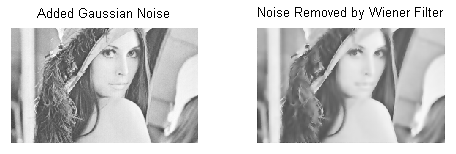
\includegraphics{Wiener.png}

\subsection{SURE-LET Approach}
	\begin{itemize}
	\item A new approach to image denoising,based on the image-domain minimization of an estimate of the
	mean squared error:
	
	\textbf{Stein's unbiased risk estimate (SURE)}
	\item The denoising process can
	be expressed as a linear combination of elementary denoising
	processes: 
	
	\textbf{Linear expansion of thresholds (LET)}
		\item  Evaluate this denoising performances by comparing \textbf{PSNR}
\end{itemize}
\textbf{$\Rightarrow$ SURE-LET Approach}

We have SURE-LET Formula as below :

$\displaystyle\sum_{l=1}^{K}\underbrace{F_k(y)^T F_l(y)a_l}_{[M]_{k,l}} = \underbrace{F_k(y)^Ty-\sigma^2div\left\{F_k(y)\right\}}_{[c]_k}$    $$for \ k = 1,2...K$$	
\begin{center}
	$\Updownarrow$ \ \ \ \ \ \ \ \ \ \ \ \ \ \ \ \ \ \ \ \ \
	
	\
	
	\textbf{Ma=c} \ \ \ \ \ \ \ \ \ \ \ \ \ \ \ \ \ \ \ \
\end{center}

\textbf{Result:}

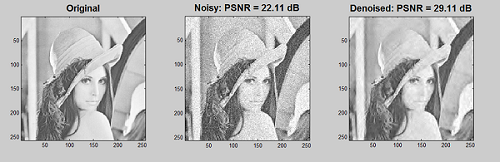
\includegraphics{surelet1.png}

\begin{itemize}
	\item Input PSNR   : 22.11[dB] 
	\item Output PSNR  : 29.11[dB]
	\item Elapsed time : 0.55[s]
\end{itemize}

With \textbf{$PSNR = 10*log_{10}(255^2/MSE)$}, we have :
\begin{itemize}
	\item Input PSNR   : 22.11[dB] \ $\Rightarrow$ Input MSE = 4.00
	\item Output PSNR  : 29.11[dB] \ $\Rightarrow$ Output MSE = 3.22
\end{itemize}
\textbf{Conclude:}

Follow SURE-LET program in Matlab, input MSE is compare between noisy image and original image, output MSE is compare between denoise image and original image. So we use output MSE result to table of Comparison Of The Results.

\section{ Comparison Of The Results }
In statistics, the mean squared error (MSE) is used to calculate the average of the squares of the errors. It mean that the difference between the estimator and what is estimated.
\begin{center}
$MSE =  \dfrac{1}{n} \displaystyle \sum_{i=1}^{n}(\hat{Y_i} - Y_i)^2$
	
\end{center}


With this report, we use Mean Error Square(MSE) to compare the original image with images use difference filter. From this, we consider about noise removal method which is the best.

The table of Comparison Of The Results as below:

\begin{center}
\begin{tabular}{|c|c|}
	\hline 
	Filter & MSE \\ 
	\hline 
	Median & 0.0372 \\ 
	\hline 
	Average & 0.0274 \\ 
	\hline 
	Gaussian & 0.0041 \\ 
	\hline 
	Weiner & 0.0372 \\ 
	\hline 
	SURE-LET & 3.22 \\ 
    \hline 
\end{tabular} 
\end{center} 


With 5 method to remove noise from images by filter. Follow results which we obtain and compare to original images. We can see result of Gaussian filter are the best of results because MSE is the smallest.






\end{document}
